\documentclass[10.5pt,a4paper]{article}
\usepackage[utf8]{inputenc}
\usepackage[T1]{fontenc}
\usepackage{lmodern}
\usepackage[margin=2.0cm]{geometry}
\usepackage{amsmath,amssymb}
\usepackage{booktabs,longtable,array,tabularx}
\usepackage{xcolor}
\usepackage{graphicx}
\usepackage[hidelinks]{hyperref}
\usepackage{fancyhdr}

\definecolor{accent}{HTML}{1F4E79}
\definecolor{soft}{HTML}{EAF1F8}
\definecolor{warn}{HTML}{FFF4E0}
\definecolor{warnline}{HTML}{C77700}

\makeatletter
\renewcommand\section{\@startsection{section}{1}{0pt}{1.3em plus .3em minus .2em}{0.4em}{\Large\bfseries\color{accent}}}
\renewcommand\subsection{\@startsection{subsection}{2}{0pt}{1.0em plus .2em minus .1em}{0.3em}{\large\bfseries\color{accent}}}
\makeatother
\setlength{\parindent}{0pt}
\setlength{\parskip}{0.4em}
\renewcommand{\arraystretch}{1.22}
\let\olditemize\itemize\renewcommand\itemize{\olditemize\setlength\itemsep{0.1em}\setlength\topsep{0.25em}}
\let\oldenumerate\enumerate\renewcommand\enumerate{\oldenumerate\setlength\itemsep{0.1em}\setlength\topsep{0.25em}}

\pagestyle{fancy}
\fancyhf{}
\fancyhead[L]{\small Meeting report: replication of Sanz et al., PRL 99, 055501}
\fancyhead[R]{\small page \thepage}
\renewcommand{\headrulewidth}{0.3pt}

\newsavebox{\mybox}
\newenvironment{keybox}{\par\medskip\noindent\begin{lrbox}{\mybox}\begin{minipage}{\dimexpr\linewidth-2\fboxsep-2\fboxrule\relax}}{\end{minipage}\end{lrbox}\noindent\fcolorbox{accent}{soft}{\usebox{\mybox}}\par\medskip}
\newenvironment{warnbox}{\par\medskip\noindent\begin{lrbox}{\mybox}\begin{minipage}{\dimexpr\linewidth-2\fboxsep-2\fboxrule\relax}}{\end{minipage}\end{lrbox}\noindent\fcolorbox{warnline}{warn}{\usebox{\mybox}}\par\medskip}

\newcommand{\Ts}{T^{*}}
\newcommand{\ps}{p^{*}}

\begin{document}

\begin{center}
{\LARGE\bfseries\color{accent} What I tried to replicate, and where it stands\\[2pt]}
{\large Brute-force NpT Monte Carlo of the oppositely charged colloid mixture at $\ps=18$}\\[3pt]
\small Target paper: Sanz, Valeriani, Frenkel, Dijkstra, \emph{Phys.\ Rev.\ Lett.} \textbf{99}, 055501 (2007)
\end{center}

\begin{keybox}
\textbf{Bottom line.} I built a signed hard-core Yukawa NpT-MC code, prepared and validated a metastable liquid at $\Ts=1$, $\ps=18$, and ran two controlled \textbf{no-swap} brute-force campaigns of $3\times10^{6}$ cycles that differ only in the particle step (dr $=0.01$ and $0.04$). \textbf{With dr $=0.04$ a close-packed crystal formed after about $2\times10^{6}$ cycles}; with dr $=0.01$ nothing nucleated. The crystal has no charge order beyond the liquid and no CsCl (bcc-type) signal, so it is a substitutionally disordered close-packed crystal, which is the \emph{qualitative} no-swap observation of the paper at $\ps=18$. Two caveats: it is a single trajectory per setting (an existence check, not a rate), and from about $2.15\times10^{6}$ cycles the crystal wraps through the periodic box, so the final size of about 500 particles is set by the box and is \textbf{not} a nucleus size. Quote the nucleation time, not the size.
\end{keybox}

%--------------------------------------------------------------------
\section{What the paper claims, and which part I targeted}

The paper tests the Stranski--Totomanow rule (the crystal with the lowest barrier nucleates). With FFS at $\ps=15$ it finds that, \emph{without} swap moves, the nuclei are disordered fcc (critical size $120\pm15$), although CsCl has the lower barrier; with 20\% swaps the nuclei become CsCl (critical size $65\pm15$). Hence sub-critical nuclei are not in equilibrium.

At $\ps=18$ the paper says only that nucleation is likely enough that \textbf{no FFS is needed}, and that plain kinetic MC without swaps forms a substitutionally disordered fcc lattice (and the same with Brownian dynamics). It gives \textbf{no cluster size, time, system size or step sizes} for this case.

\textbf{My target:} that $\ps=18$ brute-force, no-swap observation. I deliberately did \emph{not} do FFS, swap moves or umbrella sampling. Because the paper gives no numbers at $\ps=18$, the comparison is qualitative.

%--------------------------------------------------------------------
\section{What I built and how I set it up}

\begin{itemize}
\item \textbf{Code.} Started from the Frenkel--Smit Lennard-Jones NpT Fortran case study (compiled and run first), and changed the pair potential to the signed hard-core Yukawa form (like charges repel, unlike attract), with particle types, hard-core rejection and a LAMMPS trajectory output.
\item \textbf{Model.} $N=1000$ (500 positive, 500 negative), $\Ts=1$, $\ps=18$, $\kappa\sigma=6$, $r_c=3.5\sigma$. One MC cycle $=$ 1000 displacement attempts $+$ 1 volume attempt, as in the paper.
\item \textbf{Liquid preparation.} Small tests at $N=500$ first. Then, at $N=1000$, a seven-step ramp from $\Ts=2$, $\ps=5$ down to $\Ts=1$, $\ps=18$.
\item \textbf{Validated parent.} After the June runs, I found the earlier q6 cluster output unconvincing (an apparent cluster was not obvious by eye). I therefore rebuilt the workflow cleanly and validated one common liquid parent with checks independent of q6: no overlaps, exact 500:500, RDFs, structure factor, and OVITO PTM and CNA classification (all particles ``other'', no crystal). Density $1.037$, packing fraction $0.543$.
\item \textbf{Reproducibility.} Frozen executable, parent and executable hashes recorded in every manifest, runs split into 12 segments of 250\,000 cycles, completed run directories never edited.
\end{itemize}

%--------------------------------------------------------------------
\section{Parameters the paper does not give, and how I handled them}

\begin{center}
\small
\begin{tabularx}{\textwidth}{@{}>{\bfseries}l >{\raggedright\arraybackslash}X >{\raggedright\arraybackslash}X@{}}
\toprule
Parameter & What the paper says & What I did\\
\midrule
dr at $\ps=18$ & 0.01 for the initial flux, 0.04 for FFS branching; nothing for the brute-force run & ran \textbf{both}, as separate labelled branches\\
Volume step \texttt{vmax} & not given (only ``one volume move per cycle'') & tuned it, see below\\
System size at $\ps=18$ & not given & 1000\\
Cluster criterion & ``largest solid cluster'', cites ref.\ [18] & q6 first, then PTM/CNA (see caveats)\\
\bottomrule
\end{tabularx}
\end{center}

\textbf{Why \texttt{vmax} matters.} The volume step does not change the NpT equilibrium, but it changes how fast the density relaxes, so it is part of the dynamics. I treated it as an algorithmic parameter and tested it in three steps:

\begin{enumerate}
\item \textbf{2$\times$2 test (1000 cycles each)}, dr $\in\{0.01,0.04\}$ $\times$ vmax $\in\{0.001,0.0005\}$:
\begin{center}
\small
\begin{tabular}{@{}cccc@{}}
\toprule
dr & vmax & particle acceptance & volume acceptance\\
\midrule
0.01 & 0.0010 & 86.4\% & 9.3\%\\
0.01 & 0.0005 & 86.7\% & 19.6\%\\
0.04 & 0.0010 & 57.3\% & 9.5\%\\
0.04 & 0.0005 & 57.2\% & 20.5\%\\
\bottomrule
\end{tabular}
\end{center}
vmax $=0.0005$ roughly doubles volume acceptance (about 20\%) and leaves particle acceptance unchanged, with no crystal formed in any test. \textbf{It was fixed at 0.0005 for both production branches.}
\item \textbf{vmax search at dr $=0.01$} (Stages A--C, same parent, different seeds): volume acceptance falls from 45\% (vmax $0.0002$) to 10\% (0.001); the density autocorrelation time is lowest at vmax $=0.0004$ (about 51 samples, volume acceptance 26\%) versus about 83 at 0.0005.
\item \textbf{Conclusion of the search:} 0.0004 is slightly more efficient, but this is a sampling-efficiency result, not a nucleation result. \textbf{The production runs used 0.0005; 0.0004 was never used in production.}
\end{enumerate}

%--------------------------------------------------------------------
\section{Results of the 3-million-cycle campaigns}

\begin{figure}[h]
\centering
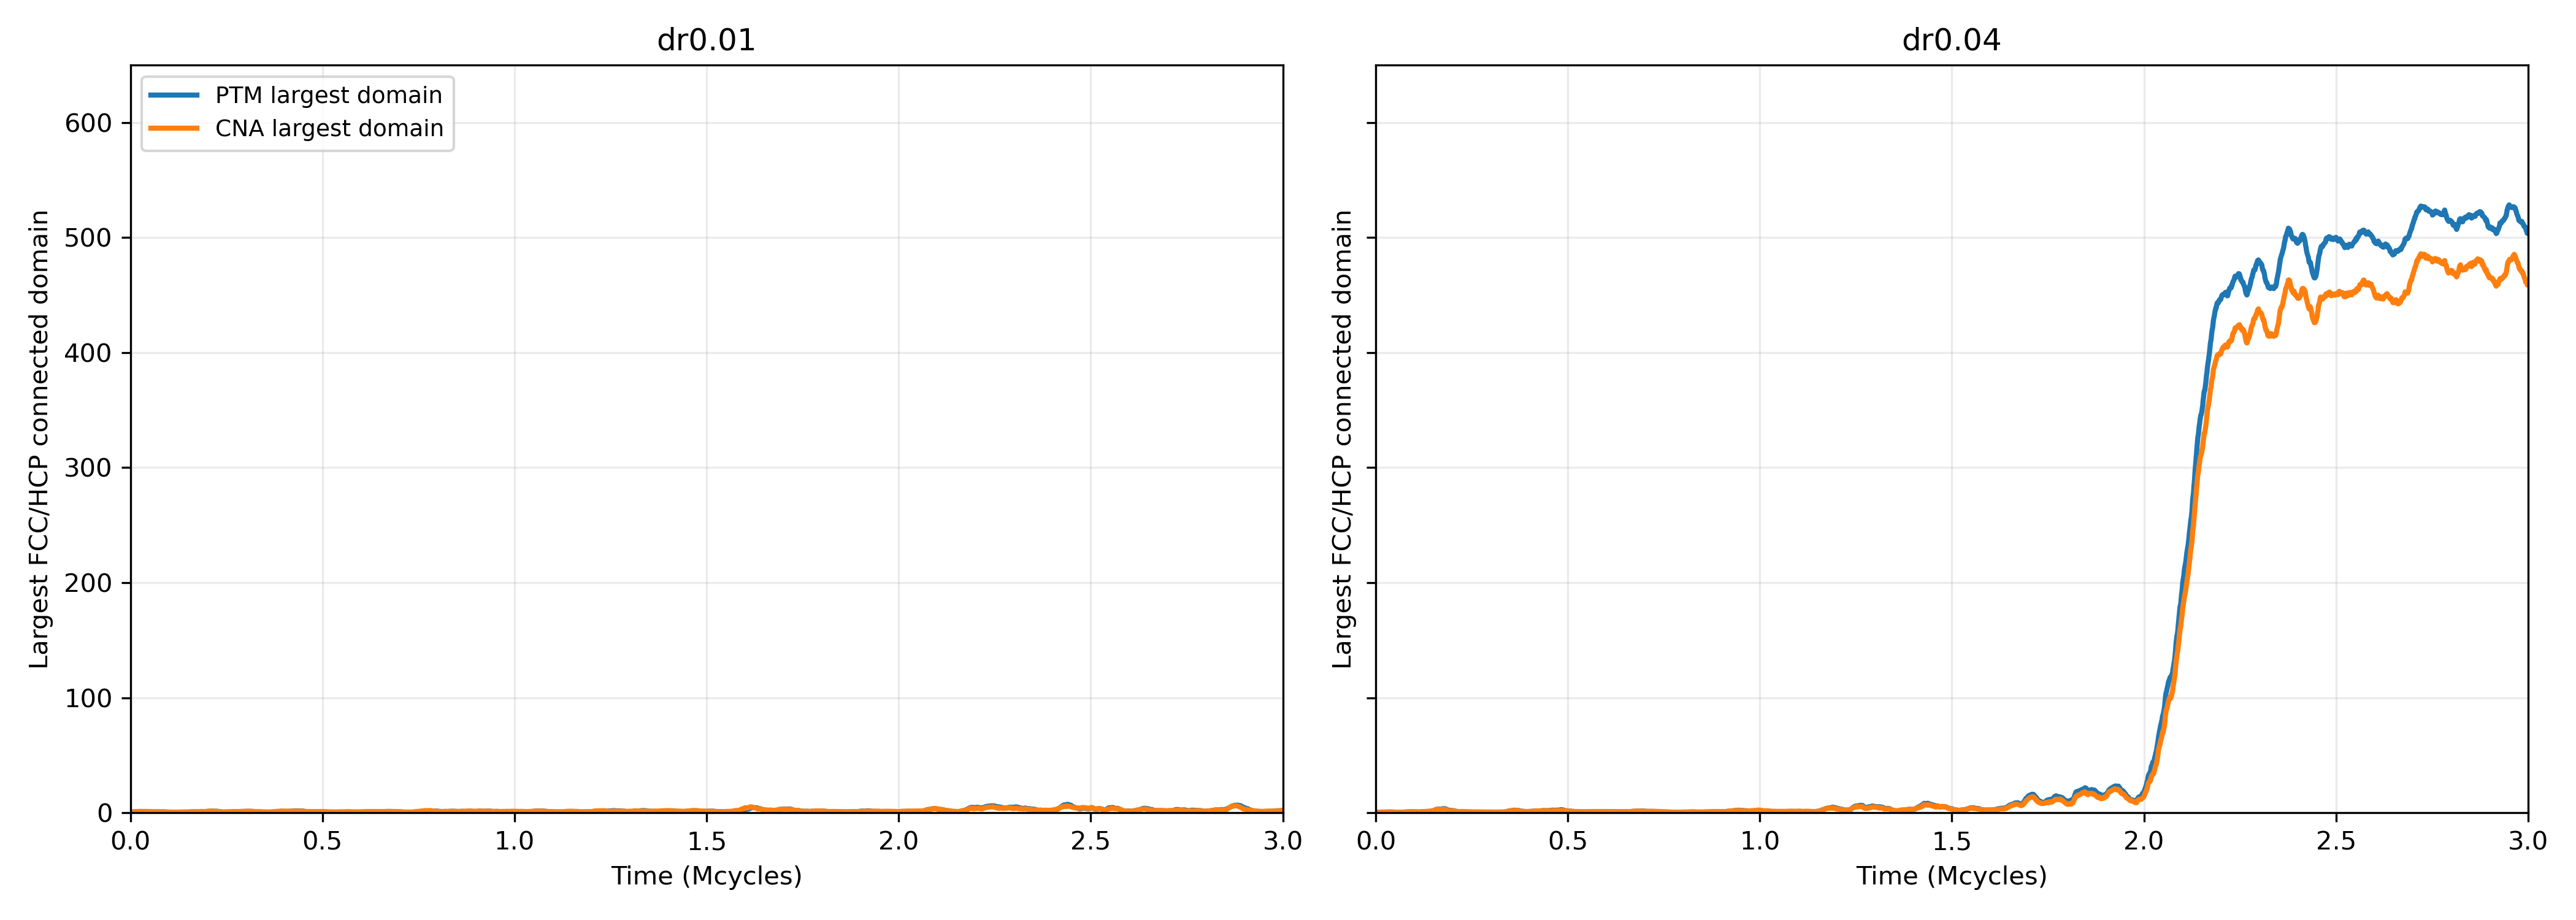
\includegraphics[width=\textwidth]{figs/largest_domain_size.png}
\caption{Largest connected fcc/hcp domain versus MC cycles (PTM and CNA), both branches started from the same liquid parent. Left: dr $=0.01$, no nucleation. Right: dr $=0.04$, a nucleus appears near $2\times10^{6}$ cycles and grows to about 500 particles. (Source: \texttt{analysis/production\_3M/largest\_domain\_size.png}.)}
\end{figure}

\begin{center}
\small
\begin{tabular}{@{}lcc@{}}
\toprule
 & dr $=0.01$ & dr $=0.04$\\
\midrule
Particle acceptance & 86.7\% & 57.4\%\\
Volume acceptance & 21.4\% & 21.9\%\\
Largest fcc/hcp domain (PTM) & $\le13$ throughout & $\approx21$ at 2.0M $\to$ 483 at 2.25M $\to$ 484 at 3.0M\\
Composition at 3.0M (PTM) & almost all ``other'' & 160 fcc, 324 hcp, 2 bcc, 514 other\\
\bottomrule
\end{tabular}
\end{center}

\textbf{Reading.} The crystal is close-packed (fcc plus hcp, i.e.\ stacking disorder) with essentially no bcc, so it is not CsCl. The fraction of opposite-charge nearest neighbours in it is 0.58, the same as in the liquid (0.60; random mixing 0.50; an ordered arrangement would give 0.67 or more), so there is no extra charge order: a substitutionally disordered close-packed crystal, consistent with the paper's no-swap result. The crystal is one connected body that wraps the periodic box in x, y and z from about $2.15\times10^{6}$ cycles, so the plateau near 500 is a finite-size limit. A q6 count (my settings) gives about 790 crystalline particles against 486 from PTM; I cannot say which is closer to the truth. Details: \texttt{06\_q6\_and\_halfbox\_check.pdf}. The larger step makes the dynamics much faster per cycle, which is why dr $=0.04$ nucleates within the run and dr $=0.01$ does not. The two branches must not be compared on the raw cycle axis.

%--------------------------------------------------------------------
\section{Caveats I will state openly}

\begin{itemize}
\item \textbf{One trajectory per branch.} There is no nucleation rate, no statistics and no estimate of the time-to-nucleation distribution.
\item \textbf{dr $=0.04$ at $\ps=18$ is my choice}, borrowed from the paper's FFS branching trajectories; the paper does not specify it for this run.
\item \textbf{The cluster definition is not the paper's.} The paper uses the ref.\ [18] q6 bond-order criterion (connection threshold 0.5, 7 connections). My q6 script used 0.70, and the clean campaign counts fcc/hcp particles from PTM, which excludes bcc. Absolute cluster sizes are definition-dependent: on one June trajectory the peak cluster ranged from 40 to 70 depending on the thresholds, and that cluster is not a crystal by PTM. The ref.\ [18] thresholds themselves call about 54 of 1000 liquid particles solid-like here (the paper says fewer than 5), while my 0.70 gives about 1.
\item \textbf{Finite size.} With $N=1000$ the crystal wraps the periodic box from about $2.15\times10^{6}$ cycles, so no nucleus size (and no comparison with the paper's 120 or 65 at $\ps=15$) can be read from these runs. A larger system would be a new simulation and was not done.
\item \textbf{Charge order checked only approximately.} The opposite-charge neighbour fraction (cutoff $1.3\sigma$, only PTM fcc/hcp particles) shows no extra order, but I did not compute a full same-charge versus opposite-charge RDF. PTM also finds about twice as much hcp as fcc, whereas the paper says fcc, so I call it ``close-packed (fcc/hcp)''. I did not reproduce the paper's g(r)-based structure assignment.
\item \textbf{No swap moves, FFS or umbrella sampling,} so the paper's central comparison (the barrier ordering) is not reproduced.
\end{itemize}

%--------------------------------------------------------------------
\section{Open questions and proposed next steps}

\begin{enumerate}
\item Look at frames of \texttt{seg008}--\texttt{seg009} in OVITO (Replicate $2\times2\times2$) to judge PTM (486) against q6 (about 790) and the q6 precursor between $1.5$ and $2.0\times10^{6}$ cycles. (The q6 vs.\ PTM comparison on the same frames is already done, see note 06.)
\item Compute a full same-charge and opposite-charge RDF of the crystal, and g(r) for comparison with the paper's fcc assignment.
\item Repeat the dr $=0.04$ run with more seeds (and, if wanted, with vmax $=0.0004$) to obtain a time-to-nucleation distribution, and with $N=2000$ or more to see an isolated nucleus.
\item Add a swap move and rerun, to test whether the structure becomes CsCl as in the paper.
\item Longer term: FFS at $\ps=15$, which is the natural link to the infRETIS project, then barriers.
\end{enumerate}

\subsection*{Likely questions}
\begin{itemize}
\item \emph{Did you reproduce the paper?} Qualitatively, for the no-swap $\ps=18$ observation, in one run. Not the rate or the barriers.
\item \emph{Why did dr $=0.01$ not nucleate?} Most likely it is simply slower per cycle (diffusion in MC scales roughly with the square of the step times the acceptance, so about an order of magnitude slower than dr $=0.04$; this is my estimate, not measured). More cycles or seeds would be needed to tell.
\item \emph{Why trust the crystal?} It grows from about 20 to about 480 particles between $2.0$ and $2.25\times10^{6}$ cycles and then persists, is classified as close-packed by two independent algorithms (PTM and CNA), and starts from a parent validated as liquid.
\item \emph{Is that the nucleus size?} No. The crystal fills and wraps the box, so the size is box-limited; only the nucleation time is meaningful.
\end{itemize}

\end{document}
